%%%%%%%%%%%%%%%%%%%%%%%%%%%%%%%%%%%%%%%%%
% fphw Assignment
% LaTeX Template
% Version 1.0 (27/04/2019)
%
% This template originates from:
% https://www.LaTeXTemplates.com
%
% Authors:
% Class by Felipe Portales-Oliva (f.portales.oliva@gmail.com) with template 
% content and modifications by Vel (vel@LaTeXTemplates.com)
%
% Template (this file) License:
% CC BY-NC-SA 3.0 (http://creativecommons.org/licenses/by-nc-sa/3.0/)
%
%%%%%%%%%%%%%%%%%%%%%%%%%%%%%%%%%%%%%%%%%

%----------------------------------------------------------------------------------------
%	PACKAGES AND OTHER DOCUMENT CONFIGURATIONS
%----------------------------------------------------------------------------------------

\documentclass[
	12pt, % Default font size, values between 10pt-12pt are allowed
	%letterpaper, % Uncomment for US letter paper size
	%spanish, % Uncomment for Spanish
]{fphw}

% Template-specific packages
\usepackage[utf8]{inputenc} % Required for inputting international characters
\usepackage[T1]{fontenc} % Output font encoding for international characters
\usepackage{mathpazo} % Use the Palatino font
\usepackage[dvipsnames]{xcolor}
\usepackage{graphicx} % Required for including images
\usepackage{amsmath}
\usepackage{booktabs} % Required for better horizontal rules in tables
\usepackage{listings} % Required for insertion of code
\usepackage{enumerate} % To modify the enumerate environment
\usepackage{ragged2e}
\usepackage{cancel}
\usepackage{MnSymbol,bbding,pifont}
\usepackage{everyhook}
\usepackage{lscape}
\usepackage{array}
\usepackage{float,graphicx}

\newcommand{\randomcolor}{%
  \definecolor{randomcolor}{RGB}
   {
    \pdfuniformdeviate 256,
    \pdfuniformdeviate 256,
    \pdfuniformdeviate 256
   }%
  \color{randomcolor}%
}

\usepackage{listings}
\usepackage[dvipsnames]{xcolor}
\definecolor{codegreen}{rgb}{0,0.6,0}
\definecolor{codegray}{rgb}{0.5,0.5,0.5}
\definecolor{codepurple}{rgb}{0.58,0,0.82}
\definecolor{backcolour}{rgb}{1,1,1}
\lstdefinestyle{mystyle}{
    backgroundcolor=\color{backcolour},   
    commentstyle=\color{codegreen},
    keywordstyle=\color{magenta},
    numberstyle=\tiny\color{codegray},
    stringstyle=\color{codepurple},
    basicstyle=\ttfamily\footnotesize,
    breakatwhitespace=false,         
    breaklines=true,                 
    captionpos=b,                    
    keepspaces=true,                 
    numbers=left,                    
    numbersep=5pt,                  
    showspaces=false,                
    showstringspaces=false,
    showtabs=false,                  
    tabsize=2
}
\renewcommand{\lstlistingname}{Código}% Listing -> Algorithm
\lstset{style=mystyle}

%----------------------------------------------------------------------------------------
%	ASSIGNMENT INFORMATION
%----------------------------------------------------------------------------------------

\title{Assignment \#3} % Assignment title

\author{Luis Alberto Ballado Aradias, David Guadalupe Cervantes Martinez} % Student name

\date{\today} % Due date

\institute{Centro de Investigación y de Estudios Avanzados del IPN \\ Unidad Tamaulipas} % Institute or school name

\class{Tecnologías Computacionales (Sep - Dec 2022)} % Course or class name

\professor{Dr. Edwyn Aldana Bobadilla} % Professor or teacher in charge of the assignment

%----------------------------------------------------------------------------------------


\begin{document}

\maketitle % Output the assignment title, created automatically using the information in the custom commands above

%----------------------------------------------------------------------------------------
%	ASSIGNMENT CONTENT
%----------------------------------------------------------------------------------------

{\color{teal}
  \dotfill
  Diagrama de Clases
\dotfill}

\begin{figure}[H]
  \centering
  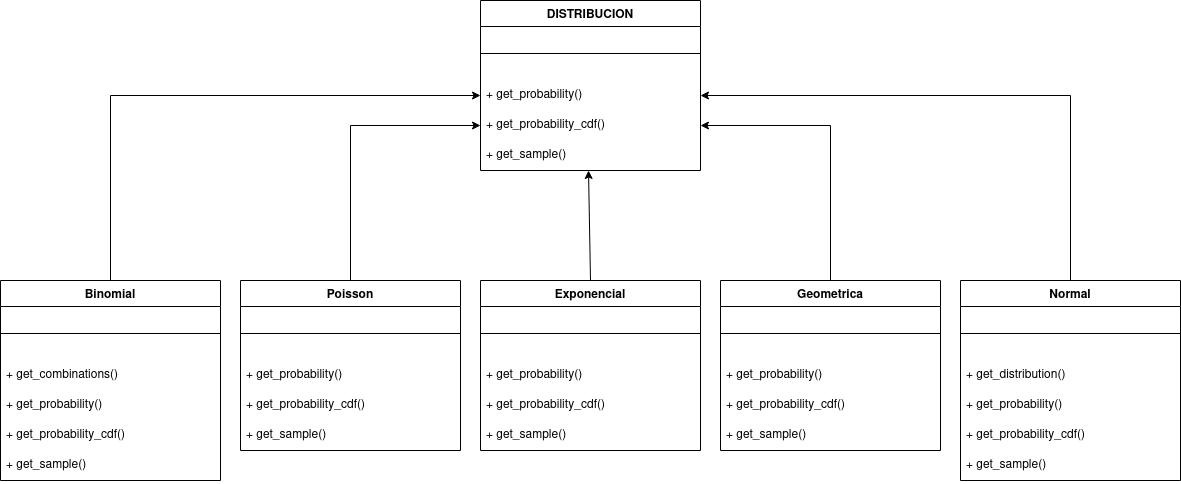
\includegraphics[scale=0.4,angle=90]{images/Diagram.png}
\end{figure}


\newpage

{\color{teal}
  \dotfill
  Vista Proyecto Dash
\dotfill}

El proyecto consta de tres archivos

\begin{itemize}
\item $server.py$ - Archivo donde se contruyen los elementos visuales con ayuda del framework Dash en python
\item $distribuciones.py$ - Archivo donde se implementa el patron factory para cinco distribuciones (Binomial, Poisson, Geometrica, Exponencial, Normal
\item $textos_distribuciones.py$ - Archivo donde existe una función que regresa textos informativos por cada distribución
\end{itemize}


{\color{teal}
  \dotfill
  server.py
\dotfill}

Al hacer uso de una extención de dash para tener acceso a componentes de tipo bootstrap se configuró lo siguiente:

\begin{lstlisting}[language=Python, caption=Configuración Dash]
  import dash_bootstrap_components as dbc # importamos el paquete

  external_stylesheets = [dbc.themes.BOOTSTRAP, dbc.icons.BOOTSTRAP] # configuramos que tome los estilos de bootstrap asi como los iconos

  app = Dash(
    __name__,
    meta_tags=[{"name": "viewport", "content": "width=device-width, initial-scale=1"}],
    external_stylesheets=external_stylesheets,
    title="Distribuciones"
  )

  app._favicon = ("assets/favicon.ico") # colocamos un favicon

  d = DistribucionFactory() # Se inicializa el objeto abstracto de las distribuciones
  
\end{lstlisting}

{\color{teal}
  \dotfill
  Componentes DASH - Dropdown (selección tipo distribución)
  \dotfill}

\begin{lstlisting}[language=Python]
# Bloque del dropdown                                                                                      
type_distribution = html.Div(
    [
        dbc.Label("Distribucion -"),
        html.I(className="bi bi-info-circle-fill me-2", id="distribucion_tooltip"),
        dcc.Dropdown(
            id="tipo_distribucion",
            options=[
                {"label": col, "value": col} for col in distribuciones
            ],
            value="Binomial",
        ),
        dbc.Tooltip("Selecciona un tipo de distribucion", target="distribucion_tooltip")
    ]
)
\end{lstlisting}
\newpage
{\color{teal}
  \dotfill
  Componentes DASH - Switch (seleccionar acumulada o no)
  \dotfill}

\begin{lstlisting}[language=Python]
# Bloque del switch                                                                                        
switches = html.Div(
    [
        dbc.Label("Acumulada -"),
        html.I(className="bi bi-info-circle-fill me-2", id="acumulada_tooltip"),
        dbc.Switch(
            id="acumulada_switch",
            value=False,
        ),
        dbc.Tooltip("Calcular la version de probabilidad acumulada", target="acumulada_tooltip")
    ]
)
\end{lstlisting}

{\color{teal}
  \dotfill
  Componentes DASH - Inputs para distribucion binomial
  \dotfill}

\begin{lstlisting}[language=Python]
# Bloque del switch                                                                                        
switches = html.Div(
    [
        dbc.Label("Acumulada -"),
        html.I(className="bi bi-info-circle-fill me-2", id="acumulada_tooltip"),
        dbc.Switch(
            id="acumulada_switch",
            value=False,
        ),
        dbc.Tooltip("Calcular la version de probabilidad acumulada", target="acumulada_tooltip")
    ]
)
\end{lstlisting}

{\color{teal}
  \dotfill
  Componentes DASH - Inputs para distribucion binomial
  \dotfill}

\begin{lstlisting}[language=Python]
# Bloque de los parametros                                                                                 
parameters_binomial = html.Div(
    [
        dbc.Label("Parametros"),
        dbc.Input(id="binom_valor_n", placeholder="numero de pruebas", type="number"),
        html.Br(),
        dbc.Input(id="binom_valor_p", placeholder="probabilidad de exitos [0-1]", type="number"),
        html.Br(),
        html.Hr(),
        dbc.Label("Generar Valores para Graficar"),
        dbc.Input(id="binom_valor_x", placeholder="cardinalidad", type="number"),
    ], style= {'display': 'none'}, id='parameters_binomial'
)
\end{lstlisting}
\newpage
{\color{teal}
  \dotfill
  Componentes DASH - Inputs para distribucion poisson
  \dotfill}

\begin{lstlisting}[language=Python]
# Bloque de parametros poisson                                                                             
parameters_poisson = html.Div(
    [
        dbc.Label("Parametros"),
        dbc.Input(id="pois_valor_mu", placeholder="numero de ocurrencias esperadas > 0", type="number"),
        html.Br(),
        html.Hr(),
        dbc.Label("Generar Valores para Graficar"),
        dbc.Input(id="pois_valor_x", placeholder="cardinalidad", type="number")
    ], style= {'display': 'none'}, id='parameters_poisson'
)
\end{lstlisting}

{\color{teal}
  \dotfill
  Componentes DASH - Inputs para distribucion geometrica
  \dotfill}

\begin{lstlisting}[language=Python]
#Bloque de parametros geometrica                                                                          
parameters_geometrica = html.Div(
    [
        dbc.Label("Parametros"),
        dbc.Input(id="geom_valor_p", placeholder="probabilidad de exito [0-1]", type="number"),
        html.Br(),
        html.Hr(),
        dbc.Label("Generar Valores para Graficar"),
        dbc.Input(id="geom_valor_x", placeholder="cardinalidad", type="number")
    ], style= {'display': 'none'}, id='parameters_geometrica'
)
\end{lstlisting}

{\color{teal}
  \dotfill
  Componentes DASH - Inputs para distribucion exponencial
  \dotfill}

\begin{lstlisting}[language=Python]

# Bloque de parametros exponencial                                                                         
parameters_exponencial = html.Div(
    [
        dbc.Label("Parametros"),
        dbc.Input(id="exp_valor_alpha", placeholder="tasa de ocurrencia del evento > 0", type="number"),
        html.Br(),
        html.Hr(),
        dbc.Label("Generar Valores para Graficar"),
        dbc.Input(id="exp_valor_x", placeholder="cardinalidad", type="number")
    ], style= {'display': 'none'}, id='parameters_exponencial'
)
\end{lstlisting}

\newpage
{\color{teal}
  \dotfill
  Componentes DASH - Inputs para distribucion normal
  \dotfill}

\begin{lstlisting}[language=Python]
# Bloque de parametros normal                                                                              
parameters_normal = html.Div(
    [
        dbc.Label("Parametros"),
        dbc.Input(id="norm_valor_mu", placeholder="media de distribucion", type="number"),
        html.Br(),
        dbc.Input(id="norm_valor_sigma", placeholder="desviacion estandar de la distribucion > 0", type="n\
umber"),
        html.Br(),
        html.Hr(),
        dbc.Label("Generar Valores para Graficar"),
        dbc.Input(id="norm_valor_x", placeholder="cardinalidad", type="number")
    ], style= {'display': 'none'}, id='parameters_normal'
)
\end{lstlisting}


{\color{teal}
  \dotfill
  Componentes DASH - Botones Aceptar / Cancelar
  \dotfill}

\begin{lstlisting}[language=Python]
# Bloque de botones                                                                                        
actions_buttons = html.Div(
    [
        dbc.Button("CANCELAR", id="cancel_btn", color="danger", className="me-1", n_clicks=0),
        dbc.Button("ACEPTAR", id="aceptar_btn", color="success", className="me-1", n_clicks=0),
        html.Span(id="example-output", style={"verticalAlign": "middle","display":"none"}),
    ],
    className="d-grid gap-2 d-md-flex justify-content-md-center",
)
\end{lstlisting}


{\color{teal}
  \dotfill
  Componentes DASH - Tarjeta con componentes
  \dotfill}

Al tener los componentes por partes, dentro de la tarjeta se agrupan de la siguiente manera

\begin{lstlisting}[language=Python]
# Tarjeta con todos los elementos                                                                          
controls = dbc.Card(
    [
        type_distribution,
        html.Br(),
        switches,
        html.Br(),
        parameters_binomial,
        parameters_poisson,
        parameters_geometrica,
        parameters_exponencial,
        parameters_normal,
        html.Br(),
        actions_buttons
    ],
    body=True,
)
\end{lstlisting}

\newpage
{\color{teal}
  \dotfill
  Componentes DASH - Grafica
  \dotfill}

Por practicidad se inicializa un componente tipo gráfica ya que es necesario que este inicializado para poder mutarlo durante el proceso de cálculos. Así también se incluye un bloque de texto informativo para cada distribución.

\begin{lstlisting}[language=Python]
# Grafica                                                                                                  
generate_graph = dcc.Graph(
    id='distribution-graph',
    mathjax=True
)
\end{lstlisting}

\begin{lstlisting}[language=Python]
# Bloque de texto                                                                                          
_latex_ = dcc.Markdown(
    children = ''' ''',
    mathjax=True,id='latex_text'
)
\end{lstlisting}

{\color{teal}
  \dotfill
   Contenedor Principal
  \dotfill}

Al tener los elementos por partes, dentro del layout en dash se incluyen las partes para formar la vista a mostrarse.
Con uso de los estilos de bootstrap en el acomodo por renglones y columnas

\begin{lstlisting}[language=Python]
# Contenedor principal                                                                                     
app.layout = dbc.Container(
    [
        html.H1("Distribuciones"),
        html.Hr(),
        dbc.Row(
            [
                dbc.Col(controls, md=4),
                dbc.Col(
                    generate_graph
                    , md=8),
            ],
            align="center",
	),
        html.Hr(),
        html.Br(),
        _latex_
    ],
    fluid=True,
)
\end{lstlisting}


\newpage

{\color{teal}
  \dotfill
  Dash - Callbacks
\dotfill}

Parte de la funcionalidad descansa en el uso de los callbacks y poder mutar la vista con la información generada \\

Callback Dropdown - Este callback controlará los elementos visibles para ser elegidos por el usuario, de manera que no todas las distribuciones tienen las mismas entradas. Se define el callback como salidas los componentes de cada distribucion y como entrada el valor del dropdown
\begin{lstlisting}[language=Python,caption=Callback dropdown]
#Callback del dropdown                                                                                     
#oculta los inputs de las distribuciones                                                                   
#que no fueron elegidos                                                                                    
@app.callback(
    Output('parameters_binomial', 'style'),
    Output('parameters_poisson', 'style'),
    Output('parameters_geometrica', 'style'),
    Output('parameters_exponencial', 'style'),
    Output('parameters_normal', 'style'),
    [Input(component_id='tipo_distribucion', component_property='value')])
def show_hide_element(value):
    if value == 'Binomial':
        return {'display':'block'},{'display':'none'},{'display':'none'},{'display':'none'},{'display':'no\
ne'}
    elif value == 'Poisson':
        return {'display':'none'},{'display':'block'},{'display':'none'},{'display':'none'},{'display':'no\
ne'}
    elif value == 'Geometrica':
        return {'display':'none'},{'display':'none'},{'display':'block'},{'display':'none'},{'display':'no\
ne'}
    elif value == 'Exponencial':
        return {'display':'none'},{'display':'none'},{'display':'none'},{'display':'block'},{'display':'no\
ne'}
    elif value == 'Normal':
        return {'display':'none'},{'display':'none'},{'display':'none'},{'display':'none'},{'display':'blo\
ck'}
    else:
        return {'display':'none'},{'display':'none'},{'display':'none'},{'display':'none'},{'display':'non\
e'}

\end{lstlisting}

\newpage
Callback de Cancelar\\

Dentro de las primeras implementaciones de los callbacks fue de un boton cancelar que limpiara los inputs cuya entrada es el evento del click, y la salida son todos los inputs de todas las distribuciones
\newpage
\begin{lstlisting}[language=Python,caption=Callback Boton Cancelar]
# Callback del boton CANCELAR                                                                              
# Limpia todos los inputs                                                                                  
@app.callback(
    Output('acumulada_switch','value'),
    Output('binom_valor_n','value'),
    Output('binom_valor_p','value'),
    Output('binom_valor_x','value'),
    Output('pois_valor_mu','value'),
    Output('pois_valor_x','value'),
    Output('geom_valor_p','value'),
    Output('geom_valor_x','value'),
    Output('exp_valor_alpha','value'),
    Output('exp_valor_x','value'),
    Output('norm_valor_mu','value'),
    Output('norm_valor_sigma','value'),
    Output('norm_valor_x','value'),
    [Input('cancel_btn', 'n_clicks')]
)
def on_cancel_click(n):
    if n is None:
        return "Not clicked."
    else:
        return False,'','','','','','','','','','','',''
\end{lstlisting}
\newpage
El callback del boton aceptar es el mas cargado ya que contiene todos los calculos de las cinco distribuciones implementadas\\

Se cuenta como entrada la accion del boton aceptar, y como salida la generacion del grafico y el texto explicativo. Se observan los estados de los diferentes inputs de las distribuciones. Al ser pulsado el boton ACEPTAR y se tenga elegida una distribucion entrara dentro de la segunda parte del if-else

\begin{lstlisting}[language=Python,caption=Callback Boton Aceptar]
# Callback del buton ACEPTAR                                                                               
# El output es la grafica                                                                                  
@app.callback(
    Output('distribution-graph', 'figure'),
    Output('latex_text', 'children'),
    Input('aceptar_btn', 'n_clicks'),
    State('tipo_distribucion','value'),
    State('acumulada_switch', 'value'),
    State('binom_valor_n','value'),
    State('binom_valor_p','value'),
    State('binom_valor_x','value'),
    State('pois_valor_mu','value'),
    State('pois_valor_x','value'),
    State('geom_valor_p','value'),
    State('geom_valor_x','value'),
    State('exp_valor_alpha','value'),
    State('exp_valor_x','value'),
    State('norm_valor_mu','value'),
    State('norm_valor_sigma','value'),
    State('norm_valor_x','value'),
)
def on_accept_click(n,tipo_distribucion,acumulada_switch,
                    binom_valor_n,binom_valor_p,binom_valor_x,
                    pois_valor_mu,pois_valor_x,
                    geom_valor_p,geom_valor_x,
                    exp_valor_alpha,exp_valor_x,
                    norm_valor_mu,norm_valor_sigma,norm_valor_x
                    ):

    if n <= 0:
        # Crear un grafico vacio                                                                           
        text = ''''''
        return go.Figure(go.Scatter(x=[0], y=[0], fill="toself")),text
\end{lstlisting}

\newpage
El cálculo de la distribución binomial descansa en la clase abstracta y el uso del DataFrame de pandas

\begin{lstlisting}[language=Python,caption=Distribucion Binomial]
    else:

        # en acumulada se deben de sumar la prob actual mas la anterior                                    

        if tipo_distribucion == 'Binomial':

            datos = {}
            datos['n'] = binom_valor_n
            datos['p'] = binom_valor_p
            datos['x'] = binom_valor_x
            datos['acumulada'] = acumulada_switch

            binomial = d.getDistribution("Binomial",datos)

            # Crear DataFrame                                                                              
            if not acumulada_switch:
                df = pd.DataFrame(binomial.get_sample(binom_valor_x),columns=['n_gen'])
                df['pdf'] = df['n_gen'].apply(lambda x: binomial.get_probability(x))
                x_axis = "X_AXIS"
                y_axis = "Y_AXIS"
            else:
                df = pd.DataFrame(binomial.get_sample(binom_valor_x),columns=['n_gen'])
                df['pdf'] = df['n_gen'].apply(lambda x: binomial.get_probability_cdf(x))
                x_axis = "X_AXIS"
                y_axis = "Y_AXIS"

\end{lstlisting}

\newpage
El cálculo de la distribución poisson descansa en la clase abstracta y el uso del DataFrame de pandas

\begin{lstlisting}[language=Python,caption=Distribucion Binomial]
        elif tipo_distribucion == 'Poisson':

            datos = {}
            datos['mu'] = pois_valor_mu
            datos['x'] = pois_valor_x
            datos['acumulada'] = acumulada_switch

            poisson = d.getDistribution("Poisson",datos)

            # Crear DataFrame                                                                              
            if not acumulada_switch:
                df = pd.DataFrame(poisson.get_sample(pois_valor_x),columns=['n_gen'])
                df['pdf'] = df['n_gen'].apply(lambda x: poisson.get_probability(x))
                x_axis = "X_AXIS"
                y_axis = "Y_AXIS"
            else:
                df = pd.DataFrame(poisson.get_sample(pois_valor_x),columns=['n_gen'])
                df['pdf'] = df['n_gen'].apply(lambda x: poisson.get_probability_cdf(x))
                x_axis = "X_AXIS"
                y_axis = "Y_AXIS"

\end{lstlisting}
\newpage
El cálculo de la distribución geometrica descansa en la clase abstracta y el uso del DataFrame de pandas

\begin{lstlisting}[language=Python,caption=Distribucion Geometrica]

        elif tipo_distribucion == 'Geometrica':

            datos = {}
            datos['p'] = geom_valor_p
            datos['x'] = geom_valor_x
            datos['acumulada'] = acumulada_switch

            geometrica = d.getDistribution("Geometrica",datos)

            # Crear DataFrame                                                                              
            if not acumulada_switch:
                df = pd.DataFrame(geometrica.get_sample(geom_valor_x),columns=['n_gen'])
                df['pdf'] = df['n_gen'].apply(lambda x: geometrica.get_probability(x))
                x_axis = "X_AXIS"
                y_axis = "Y_AXIS"
            else:
                df = pd.DataFrame(geometrica.get_sample(geom_valor_x),columns=['n_gen'])
                df['pdf'] = df['n_gen'].apply(lambda x: geometrica.get_probability_cdf(x))
                x_axis = "X_AXIS"
                y_axis = "Y_AXIS"
\end{lstlisting}

\newpage
El cálculo de la distribución exponencial descansa en la clase abstracta y el uso del DataFrame de pandas

\begin{lstlisting}[language=Python,caption=Distribucion Geometrica]
        elif tipo_distribucion == 'Exponencial':

            datos = {}
            datos['alpha'] = exp_valor_alpha
            datos['x'] = exp_valor_x
            datos['acumulada'] = acumulada_switch

            exponencial = d.getDistribution("Exponencial",datos)

            if not acumulada_switch:
                df = pd.DataFrame(exponencial.get_sample(exp_valor_x),columns=['n_gen'])
                df['pdf'] = df['n_gen'].apply(lambda x: exponencial.get_probability(x))
                x_axis = "X_AXIS"
                y_axis = "Y_AXIS"
            else:
                df = pd.DataFrame(exponencial.get_sample(exp_valor_x),columns=['n_gen'])
                df['pdf'] = df['n_gen'].apply(lambda x: exponencial.get_probability_cdf(x))
                x_axis = "X_AXIS"
                y_axis = "Y_AXIS"
\end{lstlisting}
\newpage
El cálculo de la distribución normal descansa en la clase abstracta y el uso del DataFrame de pandas, al terminar el if-else se crea el gráfico con la información generada

\begin{lstlisting}[language=Python,caption=Distribucion Geometrica]

        else:

            datos = {}
            datos['mu'] = float(norm_valor_mu)
            datos['sigma'] = float(norm_valor_sigma)
            datos['acumulada'] = acumulada_switch

            # Crear objeto distribucion normal                                                             
            normal = d.getDistribution("Normal",datos)

            if not acumulada_switch:
                df = pd.DataFrame(normal.get_sample(norm_valor_x),columns=['n_gen'])
                df['pdf'] = df['n_gen'].apply(lambda x: normal.get_probability(x))
		x_axis = "X_AXIS"
                y_axis = "Y_AXIS"
            else:
                df = pd.DataFrame(normal.get_sample(norm_valor_x),columns=['n_gen'])
                df['pdf'] = df['n_gen'].apply(lambda x: normal.get_probability_cdf(x))
                x_axis = "X_AXIS"
                y_axis = "Y_AXIS"

        # Regresar grafico de respuesta                                                                    
        fig = go.Figure()
        fig.add_trace(go.Scatter(
            x=df['n_gen'],
            y=df['pdf'],
            mode="markers"
        ))

        fig.update_layout(
            title=tipo_distribucion,
            xaxis_title = x_axis,
            yaxis_title = y_axis
        )

        return fig,texto(tipo_distribucion,acumulada_switch)
\end{lstlisting}

\newpage

{\color{teal}
  \dotfill
  Correr el servidor
\dotfill}
\begin{lstlisting}[language=Python, caption=Ejecución Server]
if __name__ == '__main__':
    app.run(host='0.0.0.0', port=5001, debug=False)

\end{lstlisting}
%----------------------------------------------------------------------------------------

\end{document}
